\documentclass[a4paper,12pt]{letter} 

\usepackage{amsmath}
\usepackage{amssymb}
\usepackage{nopageno}
\usepackage{amsmath}
\usepackage{tikz}
\usepackage{tikz-3dplot}
%\usepackage{enumitem}
% \usepackage{mathtools}
%\usepackage{eqnarray,amsmath}
\usepackage[a4paper, total={7.5in, 11.25in}]{geometry}
%\usepackage[margin=2.5cm]{geometry}
\usepackage[utf8]{inputenc}
\usepackage[T1]{fontenc}
\usepackage{lmodern}
%\usepackage{amsmath, amssymb}
\usepackage{setspace}
\setstretch{1.2}
\usepackage{pgfplots}
\pgfplotsset{compat=1.18}

\begin{document}

\begin{center}
\textbf{\huge Surface Integral of a Vector Field}
\end{center}

Let $\mathbf{F} = (F_x, F_y, F_z)$ be a vector field and $S$ a smooth oriented surface.

The surface integral (flux) of $\mathbf{F}$ through $S$ is defined as:
$$ \Phi = \iint_S \mathbf{F} \cdot d\mathbf{A}, $$
where $d\mathbf{A} = \mathbf{n}\, dA$, $\mathbf{n}$ is the unit normal vector, and $dA$ is the scalar surface element.

Computation via Parametrization \\ Let the surface be parametrized by:
  $$ \mathbf{r}(u,v) = (x(u,v), y(u,v), z(u,v)) $$

Then,
$$ d\mathbf{A} = \left( \frac{\partial \mathbf{r}}{\partial u} \times \frac{\partial \mathbf{r}}{\partial v} \right) du\,dv $$
Thus,
$$ \Phi = \iint_D \mathbf{F}(\mathbf{r}(u,v)) \cdot 
\left( \frac{\partial \mathbf{r}}{\partial u} \times \frac{\partial \mathbf{r}}{\partial v} \right) du\,dv$$

Example: Constant Vector Field

\begin{center}
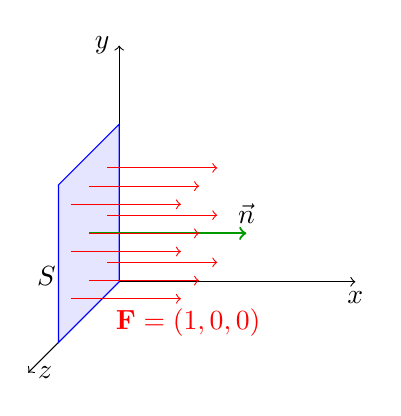
\begin{tikzpicture}[scale=2]

% Axes
\draw[->] (0,0,0) -- (1.5,0,0) node[below] {$x$};
\draw[->] (0,0,0) -- (0,1.5,0) node[left] {$y$};
\draw[->] (0,0,0) -- (0,0,1.5) node[right] {$z$};

% Square in yz-plane
\filldraw[fill=blue!10, draw=blue] 
(0,0,0) -- (0,1,0) -- (0,1,1) -- (0,0,1) -- cycle;

\node at (0,0.5,1.2) {$S$};

% Normal vector
\draw[->, thick, green!60!black] (0,0.5,0.5) -- (1,0.5,0.5);
\node[above] at (1,0.5,0.5) {$\vec{n}$};

% Vector field arrows
\foreach \y in {0.2,0.5,0.8} {
  \foreach \z in {0.2,0.5,0.8} {
    \draw[->, red] (0,\y,\z) -- (0.7,\y,\z);
  }
}

\node[red] at (0.9,0.2,1.2) {$\mathbf{F}=(1,0,0)$};

\end{tikzpicture}
\end{center}

\begin{eqnarray*}
\mathbf{F} &=& (1,0,0) \\
\mathbf{r}(u,v) &=& (0,u,v), \quad 0 \le u,v \le 1 \\
\frac{\partial \mathbf{r}}{\partial u} &=& (0,1,0), \quad
\frac{\partial \mathbf{r}}{\partial v} = (0,0,1) \\
\frac{\partial \mathbf{r}}{\partial u} &\times& 
\frac{\partial \mathbf{r}}{\partial v} = (1,0,0)\\
d\mathbf{A} &=& (1,0,0)\, du\,dv \\
\Phi &=& \int_0^1 \int_0^1 (1,0,0)\cdot(1,0,0)\, du\,dv = 1
\end{eqnarray*}



\end{document}
